\documentclass[twoside,twocolumn,10pt]{extarticle}

\usepackage{multirow}
\usepackage{textcase}
\usepackage{amsthm}
\usepackage{amssymb}
%\newtheorem{thm}{Theorem}
\theoremstyle{definition}
%\newtheorem{defn}[thm]{Definition} % definition numbers are dependent on theorem numbers
%\newtheorem{exmp}[thm]{Example}

\usepackage{blindtext} % Package to generate dummy text throughout this template 

\usepackage[sc]{mathpazo} % Use the Palatino font
\usepackage[T1]{fontenc} % Use 8-bit encoding that has 256 glyphs
\linespread{1.05} % Line spacing - Palatino needs more space between lines
\usepackage{microtype} % Slightly tweak font spacing for aesthetics

\usepackage[italian]{babel} % Language hyphenation and typographical rules
\usepackage[utf8]{inputenc}

\usepackage[hmarginratio=1:1,top=32mm,columnsep=20pt]{geometry} % Document margins
\usepackage[hang,small,labelfont=bf,up,textfont=it,up]{caption} % Custom captions under/above floats in tables or figures
\usepackage{booktabs} % Horizontal rules in tables
\usepackage{subcaption}

\usepackage{graphicx}
\usepackage{float}
\usepackage{listings}
\usepackage{color}
\usepackage{textcomp}

\definecolor{codegreen}{rgb}{0,0.6,0}
\definecolor{codegray}{rgb}{0.5,0.5,0.5}
\definecolor{codepurple}{rgb}{0.58,0,0.82}
\definecolor{backcolour}{rgb}{0.95,0.95,0.92}

\lstdefinestyle{mystyle}{
	backgroundcolor=\color{backcolour},   
	commentstyle=\color{codegreen},
	keywordstyle=\color{magenta},
	numberstyle=\tiny\color{codegray},
	stringstyle=\color{codepurple},
	basicstyle=\footnotesize,
	breakatwhitespace=false,         
	breaklines=true,                 
	captionpos=b,                    
	keepspaces=true,                 
	numbers=left,                    
	numbersep=5pt,                  
	showspaces=false,                
	showstringspaces=false,
	showtabs=false,                  
	tabsize=2
}
\lstset{style=mystyle}

\usepackage{lettrine} % The lettrine is the first enlarged letter at the beginning of the text

\usepackage{enumitem} % Customized lists
\setlist[itemize]{noitemsep} % Make itemize lists more compact

\usepackage{abstract} % Allows abstract customization
\renewcommand{\abstractnamefont}{\normalfont\bfseries} % Set the "Abstract" text to bold
\renewcommand{\abstracttextfont}{\normalfont\small\itshape} % Set the abstract itself to small italic text

\usepackage{titlesec} % Allows customization of titles
\renewcommand\thesection{\Roman{section}} % Roman numerals for the sections
\renewcommand\thesubsection{\roman{subsection}} % roman numerals for subsections
\titleformat{\section}[block]{\large\scshape\centering}{\thesection.}{1em}{} % Change the look of the section titles
\titleformat{\subsection}[block]{\large}{\thesubsection.}{1em}{} % Change the look of the section titles

\usepackage{fancyhdr} % Headers and footers
\pagestyle{fancy} % All pages have headers and footers
\fancyhead{} % Blank out the default header
\fancyfoot{} % Blank out the default footer
\fancyhead[C]{Apprendimento per Rinforzo $\bullet$ Maggio 2017 $\bullet$ \textit{Machine Leargning}} % Custom header text
\fancyfoot[RO,LE]{\thepage} % Custom footer text

\usepackage{titling} % Customizing the title section

\usepackage{hyperref} % For hyperlinks in the PDF

% Title Section
\setlength{\droptitle}{-4\baselineskip} % Move the title up

\pretitle{\begin{center}\Huge\bfseries} % Article title formatting
\posttitle{\end{center}} % Article title closing formatting
\title{Reinforcement Learning e\\ Agenti basati su Experience Replay:\\ Caso di Studio di Inefficacia} % Article title
\author{%
\textsc{Maxim Gaina e Bartolomeo Lombardi} \\[1ex] % Your name
\normalsize Università di Bologna\thanks{Progetto per il corso di Complementi di Linguaggi di Programmazione, A.A. 2016/2017, prof. Andrea Asperti.} \\ % Your institution
\normalsize \href{mailto:maxim.gaina@studio.unibo.it}{\{maxim.gaina, bartolomeo.lombardi\}@studio.unibo.it}
%\and % Uncomment if 2 authors are required, duplicate these 4 lines if more
%\textsc{Jane Smith}\thanks{Corresponding author} \\[1ex] % Second author's name
%\normalsize University of Utah \\ % Second author's institution
%\normalsize \href{mailto:jane@smith.com}{jane@smith.com} % Second author's email address
}
\date{\today} % Leave empty to omit a date
\renewcommand{\maketitlehookd}{%
\begin{abstract}
\noindent L'obiettivo di questo lavoro di progetto consiste in primo luogo nello studio di una particolare tecnica di apprendimento, detta \textit{Reinforcement Learning}. Verrà poi  applicata all'ambito ludico.
\end{abstract}
}

\begin{document}

\maketitle

\tableofcontents

\section*{Introduzione}
	\lettrine[nindent = 0.4em,lines=3]{O}\space\MakeTextLowercase{g}ni lingua 
	
\section{Agente Deep Q\texttwelveudash Network}\label{sec:dqn-agent}
	Qui (e in introduzione) descrivere Lavoro di Deep Mind.
	\theoremstyle{plain}
	\newtheorem{definition}{Definizione}
	\begin{definition}[Def]\label{def:}
		def
	\end{definition}

	\subsection{Sotto la soglia umana}
		Introdurre il problema dei giochi che non raggiungono prestazioni umane. (postare results)

\section{Reti Neurali Convoluzionali}\label{}
Le reti neurali convoluzionali (CNN) sono di fatto delle reti neurali artificiali ma differiscono in alcuni aspetti: sono costituite da neuroni collegati tra loro tramite rami pesati e i parametri allenabili anche per questa tipologia di rete sono: weight e bias. Quanto risaputo sull'allenamento di una rete neurale, cioè forward/backward propagation e aggiornamento dei weight, vale anche in questo contesto. Inoltre un'intera rete neurale convoluzionale utilizza sempre una singola funzione di costo differenziabile.
Quindi la risposta alla domanda "che cosa differisce da una comune rete neurale?" è che un'architettura CNN fa una specifica assunzione che in input ci sia un'immagine e ciò permette ad essa di assumere delle specifiche proprietà al fine di elaborare al meglio tali dati. %Ad esempio di poter effettuare delle for-ward propagation più efficienti in modo da ridurre l'ammontare di parametri della rete.
\subsection{Architettura}
Le normali reti neurali stratificate con un'architettura fully connected, dove ogni neurone di ciascun layer è collegato a tutti i neuroni del layer precedente (neuroni bias esclusi), in generale non scalano bene con l'aumentare delle dimensioni delle immagini.
Le reti neuronali convoluzionali prendono vantaggio dal fatto che l'input consiste in immagini e quindi vincolano l'architettura in modo più sensibile. In particolare, a differenza di una normale rete neurale, gli strati di un ConvNet hanno neuroni disposti in tre dimensioni: larghezza, altezza e profondità. 
Inoltre, i neuroni di un layer sono connessi solo ad una piccola regione del layer precedente, invece che a tutti i neuroni come in un'architettura fully connected. Questa è la principale caratteristica che contraddistingue una CNN da una normale rete neurale stratificata con un'architettura fully connected. In figura \ref{fig:cnn} si può vedere come vengono disposti i neuroni all'interno di una CNN, infatti ciascun layer trasforma un volume 3D di input in un volume 3D di output; quest'ultimo costituisce l'insieme delle attivazioni dei neuroni di tale layer, tramite una determinata funzione di attivazione differenziabile.
Una CNN è strutturata da tre principali layers: \textbf{Convolutional Layer}, \textbf{Pooling Layer}, e \textbf{Fully-Connected Layer}. 
\begin{figure*}[h]
\centering
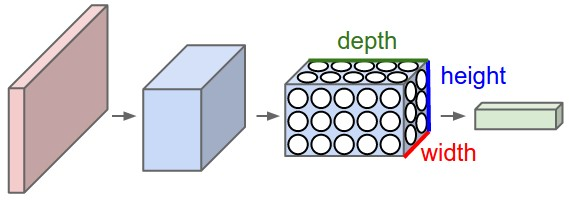
\includegraphics[scale=.4]{images/cnn.jpeg}
\caption{Rete Neurale Convoluzionale}
\label{fig:cnn}
\end{figure*}

\section{Perchè non funziona}\label{}
	\subsection{Il sospetto}
		A livello intuitivo
		\begin{table*}[h]
			\centering
			\caption{asd}
			
			\label{tab:gerarchia}
		\end{table*}
		\begin{table*}[h]
			\centering
			\caption{asd}
			\label{tab:pgm}
			
		\end{table*}
	
	
	\subsection{Perchè}
		La "dimostrazione".
		
\section{Prove}
	\subsection{Gioco successo}
	
	\subsection{Gioco fallimento}
		
\section{Agenti Alternativi}\label{}
	Spiegare l'evoluzione dell'argomento.

	\begin{figure*}[h]
		\centering
		%\includegraphics[scale=.4]{img/rnn.png}
		\caption{asd}
		\label{fig:unroll}
	\end{figure*}

	\begin{figure*}[h]
		\centering
		%\includegraphics[scale=.5]{img/lstm.png}
		\caption{asd}
		\label{fig:lstm}
	\end{figure*}

	\begin{figure*}[h]
		\centering
		\begin{subfigure}[b]{.496\textwidth}
			%\includegraphics[width=\textwidth]{img/inside-lstm.png}
			\caption{asd}
		\end{subfigure}
		\begin{subfigure}[b]{.496\textwidth}
			%\includegraphics[width=\textwidth]{img/inside-lstm2.png}
			\caption{Parametri calcolati nelle ultime fasi}
		\end{subfigure}
		\caption{asd}
		\label{fig:parmap}
	\end{figure*}
	
	\begin{equation}\label{eq:ft}
		f_t = \sigma(W_f \cdot [h_{t - 1}, x_t] + b_f)
	\end{equation}
	
	\begin{figure*}[h]
		\centering
		%\includegraphics[scale=.3]{img/seqs.jpeg}
		\caption{Problemi \textit{sequence-to-sequence} trattabili con le \texttt{RNN}}
		\label{fig:seqs}
	\end{figure*}
	\begin{figure}
		\centering
		%\includegraphics[scale=.26]{img/blstm.png}
		\caption{Architettura astratta di una rete \texttt{BLSTM}}
		\label{fig:blstm}
	\end{figure}
	\begin{figure*}[ht!]
		\centering
		\caption{Costruzione del modello con \texttt{Keras}}
		%\lstinputlisting[language=Python]{code/seq.py}
		\label{fig:modelcode}
	\end{figure*}
	\begin{table*}[]
		\centering
		\caption{Risultati ottenuti in seguito al lavoro di progetto, confrontati con il modello \texttt{LDCNF}.}
		\label{tab:results}
		
	\end{table*}
	
	\section{Conclusioni}	
	
\begin{thebibliography}{99}	
	\bibitem{bib:fenomeni-prosodici-prominenza}
		Fabio Tamburini,
		\newblock \emph{Fenomeni Prosodici e Prominenza: Un Approccio Acustico},
		2005.

	\bibitem{bib:prominence-detection-italian}
		Fabio Tamburini, Chiara Bertini, Pier Marco Bertinetto,
		\newblock \emph{Prosodic prominence detection in Italian continuous speech using probabilistic graphical models},
		2014

	\bibitem{bib:prominence-by-acoustic-analyses}
		Fabio Tamburini,
		\newblock \emph{Automatic Detection of Prosodic Prominence by Means of Acoustic Analyses},
		2015

	\bibitem{bib:chollet2015keras}
		Chollet, Fran\c{c}ois,
		\newblock \emph{Keras},
		\url{https://github.com/fchollet/keras},
		2015

	\bibitem{bib:blstm}
		Alex Graves,
		\newblock \emph{Supervised Sequence Labelling with Recurrent Neural Networks},
		2008
\end{thebibliography}

\end{document}
